\section{RISC-V ISA}

RISC-V, which stands for the fifth generation of reduced instruction set computer, was first developed by Krste Asanović in 2010 at UC Berkeley.
Unlike ARM-based microprocessors, RISC-V is an open-source ISA. Hence, it has been considered "the Linux of microprocessors".
As a matter of fact, RISC-V is a lot more than that. The groundbreaking innovation lies in its modular design.

For a long time, incremental ISA, including x86 and ARM, has been the industry convention. In other words, architects keep adding instructions but never removing for the sake of backward compatibility.  
This leads to tremendous complexity in chip design. Besides, hardware costs increase since more silicon areas are required for decode and execution of a wider variety of instructions. And most importantly,
this monolithic design approach introduces less flexibility. There is the analogy - you pay for the whole buffet, but all you want is salad.   

\section{ETISS}

ETISS, which stands for Extendable Translating Instruction Set Simulator, is developed by TUM EDA chair.
As shown in Figure~\ref{fig:etiss_structure}, it is a C++ instruction set simulator based on dynamic binary translation technique. Furthermore, it features Plugin mechanism for adding new functionalities flexibly.

\begin{figure}[htbp]
    \centering{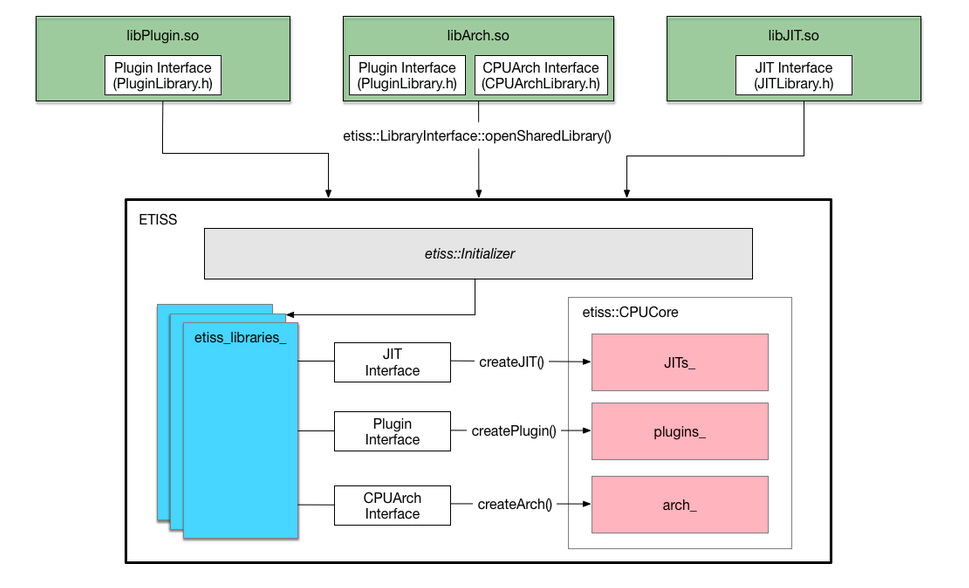
\includegraphics[scale=.4]{figures/ETISS_overview.png}}
    \caption{ETISS Structure}
    \label{fig:etiss_structure}
\end{figure}

The following will describe more details on dynamic binary translation and Plugin mechanism respectively.

\subsection{Binary Translation}
Figure~\ref{fig:etiss_binary_translation} illustrates the workflow of dynamic binary translation in ETISS.
First of all, translation block is the atomic unit in binary translator. Program counter is used to check whether the corresponding translation block exists in translation cache.
If not, instructions are fetched starting from current program counter such that a new translation block is loaded. Then, the translation block is translated into C code.
The C code snippet that represents the behaviour of all instructions in a translation block is wrapped as a function in C. The function is compiled into shared library object and cached.
Whenever it is needed, it is loaded into ETISS main loop for execution. 

% Exception handling, interrupts

\begin{figure}[htbp]
    \centering{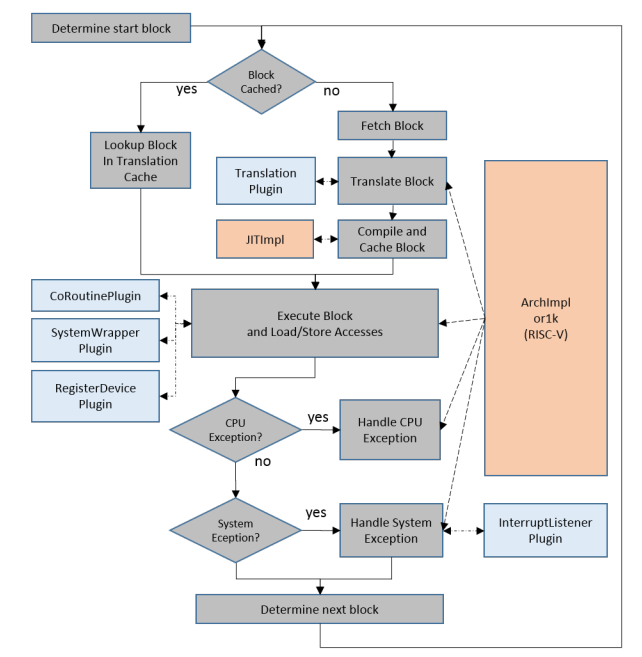
\includegraphics[scale=.45]{figures/ETISS_binary_translation.png}}
    \caption{ETISS Binary Translation}
    \label{fig:etiss_binary_translation}
\end{figure}

\subsection{Plugin Mechanism}

\section{ELF File Format}
\section{Machine Learning Deployment}
\section{Valgrind}